\section{Mathematics}

\subsection{Basic}
\subsubsection{Nomenclature}


\begin{gather*}
\begin{alignedat}{1}
    %addition
    \overbrace{
        \overbrace{
        \text{augend}+\text{addend}
        }^{\text{summands}}=\text{sum}
    }^{\text{addition}} \qquad
    %
    &
    % subtraction
    \overbrace{
        \overbrace{
        \text{minuend}-\text{subtrahend}
        }^{\text{terms}}=\text{difference}
    }^\text{subtraction}
    \\\\
    %
    % multiplication 
    \overbrace{
        \overbrace{
        \text{multiplier}\cdot\text{multiplicand}
        }^{\text{factors}}=\text{difference}
    }^\text{multiplication} \qquad
    %
    &
    % division
    \overbrace{
        \overbrace{
        \dfrac{\text{nominator}}{\text{denominator}}
        }^\text{fraction}=\dfrac{\text{dividend}}{\text{divisor}}=\text{ratio, quotient}
    }^\text{division}
\end{alignedat} \\\\
%
% expt
\overbrace{
    \text{base}^\text{exponent} = \text{power}
}^\text{exponentiation} \qquad
% sqrt
\overbrace{
    \sqrt[\text{\scriptsize degree}]{\text{radicand}}=\text{root}
}^{n\text{th root}} \qquad
% log
\overbrace{
    \log_\text{base}(\text{numerus})=\text{logarithm}
}^\text{logarithm}
\\\\
%
% absolute value
\overbrace{
    |x| = \begin{cases} x, & \text{if } x \geq 0 \\ -x, & \text{if } x < 0 \end{cases}
}^\text{absolute value} \qquad
%
% facotrial
\overbrace{
    n! = \prod_{i=1}^{n} i
}^\text{factorial} \qquad
%
% modulos
\overbrace{
    a \equiv b \pmod{n}
}^\text{modulos}
\\\\
%
% Summation
\overbrace{
    \sum_{i=m}^n a_i = a_m + a_{m+1} + \cdots + a_{n-1} + a_n
}^\text{summation} \qquad
%
% multiplication
\overbrace{
    \prod_{i=m}^n a_i = a_m \cdot a_{m+1} \cdot \cdots \cdot a_{n-1} \cdot a_n
}^\text{product of a sequence}
\\\\
%
% Derivative
\overbrace{
    f'(x) = \lim_{h \to 0} \frac{f(x+h) - f(x)}{h}
}^\text{derivative} \qquad
%
% Integral
\overbrace{
    \int_a^b f(x) dx
}^\text{integral}
\end{gather*}

\subsubsection{Greek letters}

\begin{tabular}{ccccccccc}
    \multicolumn{9}{c}{Greek Letters} \\
    Name & Alpha & Beta & Gamma & Delta & Epsilon & Zeta & Eta & Theta \\
    Lowercase & $\alpha$ & $\beta$ & $\gamma$ & $\delta$ & $\epsilon$ & $\zeta$ & $\eta$ & $\theta$ \\
    Uppercase & $A$ & $B$ & $\Gamma$ & $\Delta$ & $E$ & $Z$ & $H$ & $\Theta$ \\
    \\
    Name & Iota & Kappa & Lambda & Mu & Nu & Xi & Omicron & Pi \\
    Lowercase & $\iota$ & $\kappa$ & $\lambda$ & $\mu$ & $\nu$ & $\xi$ & $o$ & $\pi$ \\
    Uppercase & $I$ & $K$ & $\Lambda$ & $M$ & $N$ & $\Xi$ & $O$ & $\Pi$ \\
    \\
    Name & Rho & Sigma & Tau & Upsilon & Phi & Chi & Psi & Omega \\
    Lowercase & $\rho$ & $\sigma$ & $\tau$ & $\upsilon$ & $\phi$ & $\chi$ & $\psi$ & $\omega$ \\
    Uppercase & $P$ & $\Sigma$ & $T$ & $\Upsilon$ & $\Phi$ & $X$ & $\Psi$ & $\Omega$ \\
\end{tabular}

\subsubsection{Number sets}

$$
\newcommand\eq{&\,=\kern 2pt&}
\begin{alignedat}{3}
    &\mathbb{N}^+ \eq \left\{1, 2, 3,4,\dots\right\} \eq \text{Natural numbers} \\
    &\mathbb{N}_0 \eq \left\{0, 1, 2,\dots\right\} \eq \text{Whole numbers } \\
    &\mathbb{Z} \eq \left\{-1, 2, -3,\dots\right\} \eq \text{Integer numbers} \\
    &\mathbb{Q} \eq \left\{-\tfrac{4}{7}, 3,\dots\right\} \eq \text{Rational numbers} \\
    &\mathbb{R} \eq \left\{\pi, \sqrt{2},\dots\right\} \eq \text{Real numbers} \\
    &\mathbb{C} \eq \left\{a + bi \right\} \eq \text{Complex numbers}
\end{alignedat}
$$

\subsubsection{Powers, roots and logs}

\begin{gather*}
    a^{-n} = \dfrac{1}{a^n} \qquad
    a^{\frac{ b}{ c}} = \left( \sqrt[ c]{a} \space\right)^b =  \sqrt[ c]{a^b}
    \\\\
    a^n \cdot a^m = a^{m+n} \qquad
    \sqrt[n]{a}\cdot\sqrt[m]{a} = \sqrt[\uproot{15}\frac{1}{\frac{1}{n}+\frac{1}{m}}]{a} \qquad
    \log_n(a\cdot b)=\log_n(a) + \log_n(b)
    \\\\
    a^n : a^m = a^{m-n} \qquad
    \sqrt[n]{a}:\sqrt[m]{a} = \sqrt[\uproot{15}\frac{1}{\frac{1}{n}-\frac{1}{m}}]{a} \qquad    
    \log_n(a : b)=\log_n(a) - \log_n(b) 
    \\\\
    a^n \cdot b^n = \left( a \cdot b\right)^n \qquad
    \sqrt[n]{a} \cdot \sqrt[n]{b} = \sqrt[n]{a \cdot b} \qquad
    \log_n(a)\cdot\log_m(a) = \log_?(?)
    \\\\
    a^n : b^n = \left(a : b\right)^n \qquad
    \sqrt[n]{a} : \sqrt[n]{b} = \sqrt[n]{a : b} \qquad
    \log_n(a):\log_m(a) = \log_n(m)
    \\\\ 
    \left( a^n \right) ^ m = a^{m\space\cdot\space n}\qquad
    \sqrt[n]{\sqrt[m]{a}} = \sqrt[n \cdot m]{a}  \qquad
    \log_{a^n}(b^m) = \frac{m\cdot\log_a(b)}{n}
    \\\\
    x^{\log_b(y)}=b^{\log_b(x)\log_b(y)}=y^{\log_b(x)}
    \\\\
    \log_m(x) = \dfrac{\log_n(x)}{\log_n(m)}
\end{gather*}


\subsubsection{Trigonometry}

\begin{gather*}
    \sin(x) = \dfrac{O}{H} \qquad \cos(x) = \dfrac{A}{H} \qquad \text{tan}(x) = \dfrac{O}{A} \\ \space \\
    \\
    \dfrac{\text{sin}(\alpha)}{a} = \dfrac{\text{sin}(\beta)}{b}\kern 1em \text{if given angel isn't opposite to longer side} \implies \textbf{2 solutions} \\ \space \\
    \\
    c = \sqrt{a^2+b^2-2ab\cdot\text{cos}(\gamma)}
\end{gather*}

\subsection{Equations}

Indeterminate \& coefficients
$\frac{1}{x}, 2^n$ are not polynomials

Grundmenge: $\mathbb{G}$ \\
Function domain, Defintionsmenge: $\mathbb{D}$ \\
Solution set, Lösungsmege: $\mathbb{L}$ \\
\\
From the function domain we remove where the denominator is 0 or the radicand negative is
\\
Taking a root loses solutions $x^2 = 4$ because $x = 2$ loses $x = -2$ \\
For the same reason exponentiation adds solutions

Inequality invert > to < if multiplied/divided by negative numbers

For roots and absolute divide equation in positive and negative side

where $>$ becomes $<$ and for x $<$ $=>$ and, x $>$ $=>$ or

x = x 
0 = 1

\subsection{Polynomials}

\subsubsection{Lineaer}

Definition: $y = f(x) = 
\overbrace{mx+q}^\text{standard} =
\overbrace{m(x-u) + v}^\text{point}$

From $P_1(x_1,y_1)$ and $P_2(x_2, y_2)$ one can get $m = \dfrac{\Delta y}{\Delta x} = \dfrac{y_2-y_1}{x_2-x_1}$
From $m$ and $P(x, y)$ one can get $q = y-mx$
X-intersect: $x = q$
Y-intersect: $y = -\dfrac{q}{m}$
Preserve vector addition: $f(a + b) = f(a) + f(b)$
Preserve scalar multiplication: $a\cdot f(b) = f(a\cdot b)$
90° slope: $m_2 = -\dfrac{1}{m}$

\subsubsection{Quadratic}

Definition: $y = f(x) = 
\overbrace{ax^2+bx+c}^\text{standard}=
\overbrace{a(x-x_1)(x-x_2)}^\text{factored}=
\overbrace{a(x-u)^2+v}^\text{vertex}$

$x = \dfrac{-b\pm\sqrt{b^2-4ac}}{2a}$

Discriminant: $D = b^2-4ac$

%X-intersect: $\begin{rcases}
%  &x_1 = \dfrac{-b+\sqrt{D}}{2a}, x_2 = \dfrac{-b-\sqrt{D}}{2a} &\text{if } D > 0 \\
%  &x = \dfrac{-b}{2a}                                           &\text{if } D = 0 \\
%  &\varnothing                                                  &\text{if } D < 0
%\end{rcases}$
Y-intersect: $y = c$
Vertex: $S, V = P\left(-\dfrac{b}{2a}, f(x)\right) = P\left(-\dfrac{b}{2a}, -\dfrac{b^2-4ac}{4a}\right)$

- if $a > 0$, parabola opens upwards
- if $a < 0$, parabola opens downwards

\subsection{Vectors}

\newcommand\vecTwo[2]{\begin{pmatrix} #1 \\ #2 \end{pmatrix}}
\newcommand\vecThree[3]{\begin{pmatrix} #1 \\ #2 \\ #3 \end{pmatrix}}
\newcommand\abs[1]{\lvert #1 \rvert}

\begin{gather*}
\vec{v} = \vec{0v} = \vecTwo{x}{y} \\\\
\vec{AB} = \vecTwo{B_x - A_x}{B_y - A_y} \qquad \vec{BA} = \vecTwo{A_x - B_x}{A_y - B_y}\\\\
\vec{v_1} + \vec{v_2} = \vec{v_3} = \begin{pmatrix} v_{1x} + v_{2x} \\ v_{1y} + v_{2y} \end{pmatrix} \\\\
n\cdot\vec{v}=\vecTwo{n\cdot v_x}{n\cdot v_y} \\\\
\abs{a}
\end{gather*}

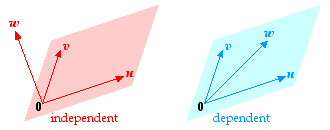
\includegraphics{./mathematics/imgs/linear.png}

A set of vectors is linearly \textbf{dependent} if one of them is \textbf{a linear combination} of the others. (or 0 because you can multiply the other by 0)
